
\chapter{多核操作系统和性能测试工具的实现}
在上一章多核操作系统可扩展性理论的基础上,本章将介绍在清华uCore实验操作系统的基础上加入对最新NUMA的多核处理器的支持,并用数种多核可扩展的数据结构和算法改造其内核数据结构。本章还介绍了本毕设设计了新型性能测试工具QProf的原理。

\section{uCore多核硬件抽象层}
uCore是清华大学研发的一个硬件平台的、遵循简化Posix标准的实验操作系统。在部分硬件平台(如ARM)上,uCore对uclibc和
bionic
C两种标准C库有较为完整的支持。但一直以来此内核都缺少对多核平台架构的支持。本毕设的一项重要工作是为uCore操作系统内核增加AMD64多核架构支持。

\subsection{概述}
uCore作为一个实验操作系统内核,包含了现代操作系统中各个主要组成部分。与Linux等主流开源操作系统类似,uCore把内核代码分为硬件无关代码(如进程管理、调度器)和硬件相关代码(包括一级硬件中断处理,硬件初始化等)。这两部分代码之间由硬件抽象层(HAL)连接,此代码层保证了uCore可以在多种硬件平台上方便地移植。事实上,现在uCore实验操作系统已经可以在i386、ARM、MIPS等平台上正常工作。但一直以来,此内核都未加入对SMP或NUMA平台的完善支持。本毕设的一项重要内容是在uCore中加入了较为健全的NUMA抽象层,并在实现了对AMD64多核硬件平台的支持。而对SMP多核系统,可以看做是NUMA架构中NUMA节点数为1的特例,在本毕设的多核硬件抽象中可以得到自然的统一的支持。

为了使uCore可以支持多核硬件平台,本毕设对硬件无关代码也加入了相关扩展。加入NUMA支持后的内核硬件无关层代码结构如表\ref{tab:ucore-common}所示。
通过把与硬件无关的多核支持相关代码与硬件特定代码分离,可以大大减少未来其他加入其他多核硬件架构(如多核ARM平台)支持的工作量。

\begin{table}[ht]
  \centering
  \caption{uCore硬件无关部分代码结构}
  \label{tab:ucore-common}
    \begin{tabular*}{\linewidth}{lp{10cm}}
      \toprule[1.5pt]
      {\heiti 目录} & {\heiti 描述} \\\midrule[1pt]
arch & 硬件相关代码,见下表 \\
fs      & 虚拟文件系统(VFS)和SFS、FAT、YAFFS文件系统支持\\
kmodule       &  内核可加载模块支持 \\
libs             & 工具函数,简化的C环境 \\
mm             & 虚拟内存管理子系统\\
module       & Linux Device Environment \\
numa           & NUMA多核架构HAL支持 \\
process        & 进程管理子系统 \\
schedule      & 调度算法,包含Round-Robin和多级返回队列算法 \\
sync              &  进程间通讯子系统 \\
syscall         & 类Unix系统调用实现 \\
sysconf        &   硬件配置信息抽象 \\
      \bottomrule[1.5pt]
    \end{tabular*}
\end{table}

另一方面,对于特定的硬件平台,需要大量硬件相关代码支持操作系统的正常运作。如对于多核AMD64架构,需要高级配置和电源管理接口(ACPI)和高级可编程中断控制器(APIC)等复杂硬件驱动来完成系统拓扑结构读取、应用处理器(Application Processor)启动以及CPU核间通讯等任务。这部分代码被封装在arch/amd64目录下,此目录的结构
如表\ref{tab:ucore-amd64}所示。

\begin{table}[ht]
  \centering
  \caption{uCore硬件相关部分(AMD64)主要代码结构}
  \label{tab:ucore-amd64}
    \begin{tabular*}{\linewidth}{lp{8cm}l}
      \toprule[1.5pt]
      {\heiti 目录} & {\heiti 描述} & {\heiti 代码行数}\\\midrule[1pt]
debug  &  硬件相关调试工具 & 304 \\
driver &    硬件驱动,本毕设实现了ACPI、IOAPIC、LAPIC等多核OS必须的驱动  &
3087 \\
init  & 内核初始化代码,包括Boot CPU和AP进入长模式的启动代码 & 568\\
libs  &  AMD64上自旋锁、GDT等硬件相关函数 & 1099 \\
mm &   支持NUMA系统的物理页管理系统 & 2328 \\
numa & AP初始化和核间通讯模块 & 265 \\
trap & 硬件中断、CPU核间中断处理 & 2026 \\
      \bottomrule[1.5pt]
    \end{tabular*}
\end{table}

\subsection{主要数据结构}

从图\ref{fig:numa-node}可以看出NUMA结构的复杂性:对于每个CPU来说,内存空间分为本地内存和远程内存,CPU访问远程内存的请求必须经过相关硬件进行中转。
换言之,与传统SMP结构不同,CPU访问不同物理内存地址所需时间可能不相同。因此,操作系统的物理内存管理系统必须认识都NUMA系统的这种特性,才能
为各个CPU高效地分配内存。另外,NUMA系统的这种特性也增大了线程迁移(migration)的开销,对调度器提出了新要求。

\begin{figure}[ht]
\centering
\begin{tikzpicture}


% Define block styles used later
\tikzstyle{ann} = [above, text width=5em, text centered]
\tikzstyle{wa} = [sensor, text width=4em, fill=red!20,
    minimum height=3em, rounded corners, drop shadow]
\tikzstyle{sc} = [sensor, text width=13em, fill=red!20,
    minimum height=10em, rounded corners, drop shadow]
\def\blockdist{2.3}
\def\edgedist{2.5}

    \node (wa) [wa]  {Router};
    \path (wa.west)+(-4.2,1.5) node (asr1) [sensor] {$P_0$};
    \path (asr1.east)+(0.6,0) node (asr2)[sensor] {$P_1$};
    \path (asr2.east)+(0.6,0) node (asr3)[sensor] {$\dots$};
    \path (asr3.east)+(0.6,0) node (asr4)[sensor] {$P_n$};
    \path (asr1.south)+(1.8, -1) node (mem0) [sensor, text width=6em] {$Ram_0$};

    \path (mem0.south) +(0,-0.5) node (node0) {$NUMA-Node_0$};

    \begin{pgfonlayer}{background}
        \path (asr1.west |- asr1.north)+(-0.5,0.3) node (a) {};
        \path (wa.south -| wa.east)+(+0.5,-0.3) node (b) {};
        \path (asr4.east |- node0.south)+(+0.5,-0.5) node (c) {};

        \path[fill=yellow!20,rounded corners, draw=black!50, dashed]
            (a) rectangle (c);
        \path (asr1.north west)+(-0.2,0.2) node (a) {};

    \end{pgfonlayer}

    \path (wa.east)+(0.7,1.5) node (asr5) [sensor] {$P_{n+1}$};
    \path (asr5.east)+(0.6,0) node (asr6)[sensor] {$P_{n+2}$};
    \path (asr6.east)+(0.6,0) node (asr7)[sensor] {$\dots$};
    \path (asr7.east)+(0.6,0) node (asr8)[sensor] {$P_{m}$};
    \path (asr5.south)+(1.8, -1) node (mem1) [sensor, text width=6em] {$Ram_1$};

    \path (mem1.south) +(0,-0.5) node (node1) {$NUMA-Node_1$};

    \begin{pgfonlayer}{background}
        \path (asr5.west |- asr5.north)+(-0.5,0.3) node (a) {};
        \path (wa.south -| wa.east)+(+0.5,-0.3) node (b) {};
        \path (asr8.east |- node1.south)+(+0.5,-0.5) node (c) {};

        \path[fill=yellow!20,rounded corners, draw=black!50, dashed]
            (a) rectangle (c);
        \path (asr1.north west)+(-0.2,0.2) node (a) {};

    \end{pgfonlayer}


\end{tikzpicture}
\caption{HAL层NUMA拓扑结构表示}
\label{fig:numa-node}
\end{figure}

正如上面所述,NUMA平台与传统SMP架构的最大区别是CPU、内存和中断分发的复杂拓扑结构。其中CPU和物理内存间的关联性是本质区别,如图\ref{fig:numa-node}。
为了表示这种拓扑结构,本毕设在内核中维护一系列数据结构,保证内核代码可以在$O(1)$时间内响应关于系统拓扑结构的各种查询。

uCore中NUMA拓扑结构相关关键数据结构如下:
\begin{itemize}
\item \emph{struct sysconf\_s}  \pozhehao 记录了系统NUMA节点数、CPU数等统计信息;
\item \emph{struct numa\_node} \pozhehao NUMA节点对象,记录了特定NUMA节点的硬件ID、包含的CPU、内存地址分为,
	相当于图\ref{fig:numa-node}中的NUMA-Node;
\item \emph{struct cpu} \pozhehao 多核系统中最关键的数据结构之一,对每个物理CPU,都有一个对于的cpu对象。除了保存本CPU所述NUMA节点
等拓扑信息之外,还保存了本CPU的状态,如percpu变量的基地址、CPU内核栈基地址等信息;
\item \emph{struct numa\_mem\_zone} \pozhehao NUMA内存节点对象,主要保存一个指向物理页元数据链表的头指针。物理内存分配器通过这个
对象找到适当的内存节点分配内存。
\end{itemize}

本节详细叙述了uCore操作系统内核的多核硬件抽象层支持,为硬件平台特定代码的实现构建好框架。下一节将介绍在此框架上加入对AMD64 NUMA架构硬件的具体支持。


\section{AMD64多核NUMA架构硬件支持的实现}
本毕设在实验操作系统内核uCore的硬件抽象层基础上,加上了相对完整的x86\_64
NUMA多核架构支持。本内核已经在QEMU软件模拟器、KVM硬件虚拟化平台和支持ACPI的Intel真实机器上测试通过。
本节对实现过程中的重点和难点做简要介绍。

\subsection{ACPI支持}
为了支持多核CPU和NUMA结构,操作系统在启动的前期必须通过某种方式读取系统的拓扑结构信息,这些信息包括但不限于:
\begin{itemize}
\item CPU和LAPIC的关联信息
\item LAPIC和IOAPIC的连接信息
\item 物理内存和NUMA节点的关联信息
\item PCI、PCIe子系统信息
\end{itemize}

对于AMD64多核架构(如图\ref{fig:mp-arch}所示),这些拓扑信息由主板上的ACPI模块管理。在主板出厂前,硬件厂商把硬件的部分拓扑结构信息写入Firmware中的
	ACPI表。OS通过读取此表,NUMA节点等信息。上电自检后,BIOS把系统拓扑信息记录到ACPI表,并把它映射到预先定义好的内存地址上,操作系统通过读取这些信息表,即可获得当前系统的配置信息。现时uCore中用到的ACPI信息表如表\ref{tab:acpi}所示,各表项的具体结构见文献\cite{acpica}。这些表为uCore操作系统提供了NUMA节点和CPU、内存关联性等必要信息。

\begin{figure}[ht]
\begin{center}
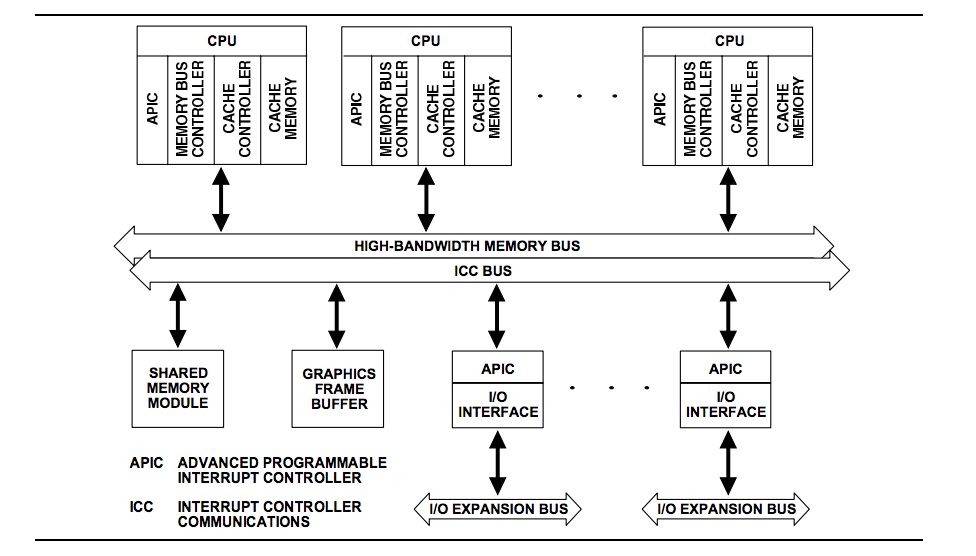
\includegraphics[width=0.7\textwidth]{figures/mp_arch.png}
\end{center}
\caption{多处理器系统架构图\cite{intelmp}}
\label{fig:mp-arch}
\end{figure}

\begin{table}[ht]
  \centering
  \caption{ACPI主要硬件信息表}
  \label{tab:acpi}
    \begin{tabular*}{\linewidth}{lp{8cm}}
      \toprule[1.5pt]
      {\heiti 表名} & {\heiti 描述} \\\midrule[1pt]
RSDT & Root System Description Table \\
MADT  & Multipile ACPI Description Table \\
SLIT    &  System Locality Distance Information Table\\
SSDT    & Secondary System Description Table\\
SRAT    & System Resource Affinity Table \\
      \bottomrule[1.5pt]
    \end{tabular*}
\end{table}


由于ACPI子系统及其信息表的复杂性,Intel公司及其他厂商发布了名为ACPI Component Architecture的开源框架,给出了与ACPI硬件规范对应的软件驱动实现。
此框架被设计为易于整合到操作系统内核的独立子系统,操作系统(如Linux和uCore)只需实现ACPICA框架中定义好的OS服务层,提供内存管理、内核线程调度
等基本接口函数,即可直接使用ACPICA框架操作ACPI兼容的硬件平台。现时,本毕设已经把ACPICA整合到uCore的编译系统中,实现了必要的OS服务层接口,
可以直接使用ACPICA的API操作硬件。

\subsection{多核中断和IPI中断支持}
AMD64多核系统的分布式中断系统如图\ref{fig:mp-arch}所示,外部硬件中断先传递到IOAPIC上,操作系统可以通过对IOAPIC的编程,实现硬件中断的路由。在uCore现时
的实现中,采用了与Linux默认配置相似的处理方法,即把绝大多数外部硬件中断路由到CPU0上,由$CPU_0$统一处理。值得注意的是,在APIC体系结构中,时钟中断不再
由外部硬件触发,而是由集成在各个CPU核中的LAPIC中。因此,每个CPU都相应各自产生的时钟中断,各个中断之间不保证同步。换言之,在Refcache(见\ref{subsec:refcache})等需要时钟同步的分布式算法中,需要软件实现时钟同步。

在多核系统上,各个CPU除了使用Cache一致共享内存的方式通讯,还可以以Message-Passing的方式通讯。在AMD64多核系统中,这种通讯方式一般用核间中断(IPI)的方式实现。
IPI中断是一种特殊的硬件中断,操作系统可以对LAPIC进行编程,向任意CPU内核发起IPI请求。在uCore中,每个CPU核有自己的IPI请求队列。当$CPU_A$需要向$CPU_B$发送IPI请求,$CPU_A$先把请求的数据和回调函数指针发到$CPU_B$的请求队列中,然后向$CPU_B$发起IPI中断,最后$CPU_B$在其中断处理例程中检查自己的IPI请求队列,并执行请求。此过程如图\ref{fig:ipi-uml}所示。

\begin{figure}
  \centering

\begin{sequencediagram}
\newthread{a}{:$CPU_A$} 
\newinst[2]{q}{:$Queue_B$}
\newthread[gray]{b}{:$CPU_B$}

\begin{call}{a}{add\_request()}{q}{}
\end{call}

\mess{a}{IPI}{b}

\begin{sdblock}{Loop}{poll rqs}
\begin{call}{b}{get\_request()}{q}{} 
\end{call}
\end{sdblock}

\mess{b}{done}{a}

\end{sequencediagram}
\label{fig:ipi-uml}
\caption{IPI处理过程UML图}
\end{figure}


\subsection{AP启动}
AMD64多核系统启动与单核系统的主要区别在于应用处理器的启动。AMD64多核系统中,上电后只有一个CPU开始正常运行,这个CPU被称为Bootstrap CPU(BSP),其他CPU处于halt状态,这些CPU被称为Application Processor(AP)\cite{intelmp}。多核操作系统启动主要分为两个阶段:

	\begin{enumerate}
		\item 系统上电后,只有Boot CPU开始工作,Boot
	CPU负责在OS启动的最后阶段唤醒Application Processor
	(AP)。这项工作根据Intel Multiprocessor规范,通过LAPIC发送
	Startup中断实现。

		\item Boot CPU把所有AP唤醒后,打开本地中断,开始正常运行。内核
	调度器开始工作,每个CPU从各自的工作队列中按照某种顺序取出Task运行。
	\end{enumerate}


如上所述,Boot CPU在内核各个子系统初始化完成之后,由Boot CPU发送IPI中断到各个应用处理器,使之开始工作。应用处理器对应的LAPIC在收到IPI中断后,重置对应的CPU使之进入实模式状态。AP启动流程与BSP启动流程大致相同:

\begin{enumerate}
\item AP从实模式进入32bit保护模式,再进入64bit长模式(Longmode)
\item 初始化本地GDT
\item 初始化GS、FS段寄存器(见\ref{subsec:percpu})
\item 加载启动页表
\item 本地IDT和中断控制器初始化
\item 本地Idle内核线程初始化
\item 开启本地中断,开始调度
\end{enumerate}

所有AP打开中断进入正常主循环后,系统启动完成。

\section{多核操作系统基础设施实现}
本节介绍uCore中为多核系统特别优化的部分数据结构的实现。

\subsection{无锁数据结构的实现}
一直以来,操作系统常用互斥锁保护链表、平衡树等数据结构。但是,这种数据结构难以在多核系统上达到较佳的可扩展性。今年来,有研究者\cite{Fraser:2007:CPW:1233307.1233309}提出使用硬件比较-交换指令(compare-and-swap,CAS)构成堆栈、链表和无锁跳表等数据结构。使用这类无锁数据结构可以避免使用粒度较大的互斥锁对整个数据结构进行保护,减少出现锁竞争的机会。但是,无锁数据结构并不保证内核的多核可扩展性,例如在多核操作系统的VM子系统使用无锁跳表管理虚拟地址区域(VMA)元数据会带来严重的Cache竞争\cite{radixvm:eurosys13},反而影响系统性能。

uCore中实现了无锁堆栈,可以用在Slab分配器中可以管理空闲页链表(Freelist)。无锁堆栈共支持三种操作:初始化init、压栈push和弹出栈顶pop,数据结构定义如下:

\begin{lstlisting}
struct lockfree_stack_entry{
	volatile struct lockfree_stack_entry *link;
};

struct lockfree_stack{
	volatile struct lockfree_stack_entry *top;
	/* avoid ABA problem */
	unsigned long volatile oc;
	atomic_t count;
};
\end{lstlisting}

为了实现push和pop操作需要使用CAS指令切换栈顶指针(lockfree\_stack中的top指针)。实现无锁数据结构的一个常见问题是所谓ABA问题\cite{Fraser:2007:CPW:1233307.1233309}。对于无锁栈,为解决ABA问题的方法使用了堆栈修改计数器oc,并在pop堆栈项操作中,修改栈顶的同时修改计数器oc(这在AMD64上使用16字节CAS指令完成)。使用这种方法,pop函数可以通过跟踪lockfree\_stack结构中top指针的``版本号'',避免ABA问题。

\subsection{支持NUMA的物理页分配器}
为了高效支持对NUMA架构,uCore中实现了一个基于非连续内存模型多核物理页分配器。此物理页分配器包括以下几个组成部分:
\begin{itemize}
	\item 内存拓扑检测
	\item 对每个NUMA节点,初始化各自的伙伴系统分配器(Buddy System)
	\item
		NUMA节点内存分配策略,如果当前节点有足够的空闲内存,在本节点上分配物理页,
		若当前节点内存不足,则应该尝试使用其他节点的物理页(这可能降低系统性能)
\end{itemize}

在NUMA系统上实现高效的物理页分配器是复杂的,现在uCore的实现中未考虑NUMA节点见的距离(这个信息可以从ACPI的SLIT表中获得)。对uCore上物理内存分配器的一个改进是,通过NUMA节点距离信息,从距离本CPU节点最近的NUMA内存节点上分配内存。

\subsection{percpu变量实现}
\label{subsec:percpu}

与用户态编程中的线程本地存储(Thread Local Storage)类似,多核操作系统内核运行过程中,对每个CPU,需要分配其私有存储空间来存储各个CPU独有的状态信息,例如本CPU上真正执行的线程控制块指针current。在多核系统中使用percpu变量的一个好处是可以避免多CPU读写同一个内存地址,造成Cache一致性协议开销,提高系统的可扩展性。
在uCore中,CPU0占用percpu变量空间在内核镜像中静态分配,保证内核在启动时可以尽早使用BSP的percpu变量存储空间。AP的percpu变量空间在启动过程中由BSP动态地在其所在NUMA节点上分配,保证AP访问percpu变量的高效性。


\begin{figure}[ht]
\centering
\begin{tikzpicture}[->,>=stealth']
\tikzstyle{mem}=[draw, fill=green!20, text width=5em,
    text centered, minimum height=2.5em,drop shadow]
\tikzstyle{LabelStyle}=[right]

\path   node (cpu0) [sensor]  {$P_0$};
\path  (cpu0.east)+(2,0) node (cpu1) [sensor]  {$P_1$};
\path  (cpu1.east)+(2,0) node (cpu2)  {$\dots$};
\path  (cpu2.east)+(2,0) node (cpun) [sensor]  {$P_n$};

\path (cpu0.center)+(0,-2) node (p0) [mem, fill=yellow!20] {$CPU_0 vars$};
\path (cpu1.center)+(0,-2) node (p1) [mem] {$CPU_1 vars$};
\path (cpu2.center)+(0,-2) node (pdot)  {$\dots$};
\path (cpun.center)+(0.,-2) node (pn) [mem] {$CPU_n vars$};

\path (cpu0) edge   node {$GS$} (p0);
\path (cpu1) edge   node {$GS$} (p1);
\path (cpun) edge   node {$GS$} (pn);

\path (p1.south)+(0,-1) node (ptr) [mem, text width=8em, fill=yellow!20] {$percpu\_offsets[]$};

\path (ptr) edge   node {} (p0);
\path (ptr) edge   node  {} (p1);
\path (ptr) edge   node  {} (pn);

\end{tikzpicture}

\caption[percpu变量的实现]{percpu变量的实现}
\label{fig:percpu-impl}
\end{figure}

本毕设percpu变量实现设计如图\ref{fig:percpu-impl}所示。 图\ref{fig:percpu-impl}中黄色部分内存在内核镜像上静态分配,绿色部分内存在各自的NUMA节点上动态分配。下面以一个percpu变量$ticks$为例,说明
uCore中percpu变量的工作原理:
\begin{enumerate}
\item
在适当的初始化后,各CPU可以通过GS段寄存器访问自己的cpu结构体:
\begin{lstlisting}
static inline struct cpu* mycpu(void){
	uint64_t val;
	asm volatile("movq %%gs:0, %0" : "=r" (val));
	return (struct cpu *)val;
}
\end{lstlisting}

\item
从cpu结构体中id成员变量可以获得本CPU的ID号,用此ID作为索引,在percpu\_offsets数组中获取本CPU percpu变量内存区域基地址的指针。

\item 由于链接器已经计算好了CPU0上$ticks_0$的地址$Addr(ticks_0)$,通过下式计算$CPU_k$上ticks的地址:
\begin{equation}
\label{eq:percpu}
ticks_k = percpu\_offsets[k] + ( Addr(ticks_0) - percpu\_offsets[0] )
\end{equation}

\end{enumerate}


\subsection{可扩展引用计数器的实现}
\label{subsec:refcache}

本毕设在\ref{sec:counter}介绍了引用计数器的建模,并得出引用计数器在多数情况下是可以通过可扩展方式实现的。本节将介绍uCore中实现的一种可扩展引用计数算法。

为了解决原子加减操作在多核系统上的可扩展性瓶颈,研究界如sloppy
counters\cite{linux:osdi10}, Scalable NonZero Indicators\cite{Ellen:2007:SSN:1281100.1281106}
等可扩展计数器。它们的基本思路都是把全局计数器分解成$N$个CPU私有计数器(存储相对于全局计数器的增量),只有当需要获取计数器真实值时才发起核间通讯,把所有私有计数器相加。本毕设在uCore的基础设施上实现了一种新型可扩展计数器Refcache\cite{radixvm:eurosys13}。Refcache相对与其他算法相比,优势是使用了类似CPU
Cache的思想,在每个核上Refcache使用的空间是常数(不随使用的计数器个数增加)。

Austin等人\cite{radixvm:eurosys13}提出的Refcache计数器主要有如下四个操作:

\begin{itemize}
	\item $inc()$ 操作,CPU本地计数器加一
	\item $dec()$ 操作,CPU本地计数器减一
	\item $evict()$
		操作,当Cache中的哈希表项出现碰撞时,把旧表项中的计数增量加到全局计数器中。
		若发现对象引用计数的真实值变为零,调用回调函数释放内存
	\item $flush()$
		操作,把CPU中的所有增量Cache应用到全局计数器中,并无效化所有增量Cache
\end{itemize}

	以上四个操作中,前两个操作(使用最频繁的操作)执行时只需要关闭内核抢占即可,无需核间同步。后两个操作尽管需要自旋锁保护关键代码段,但是当增量Cache足够大时(或哈希冲突频率足够小),它们只由时钟中断以一定频率(如每10毫秒一次)调用,对系统性能影响不大。

	本毕设实现了两个版本的Refcache(见表\ref{tab:refcache-lines}),一个是基于uCore的内核态实现,另一个是Ruby实现的用户态Refcache,用于研究其性质。

\begin{table}[ht]
  \centering
  \caption{Refcache实现}
  \label{tab:refcache-lines}
    \begin{tabular*}{\linewidth}{lll}
      \toprule[1.5pt]
      {\heiti 文件} & {\heiti 描述} & {\heiti 行数} \\\midrule[1pt]
      refcache.h & 内核态C实现 & 71 \\
      refcache.c & 内核态C实现 & 237 \\
      \hline
	refcache.rb & 用户态Ruby实现 & 113 \\
      \bottomrule[1.5pt]
    \end{tabular*}
\end{table}



\section{基于QEMU的全系统性能采集工具QPROF}
为了在模拟器中方便地寻找操作系统内核的瓶颈,本毕设这种方法结合了Qemu和gprof的两个开源软件,实现了一个全系统的Profiler
\pozhehao
QProf\footnote{https://github.com/chyh1990/qemu/tree/1.3-profiler}。

由于真实操作系统工作环境的复杂性,很难通过分析源代码等静态分析方法发现内核中的性能问题。
本全系统性能测试工具通过动态分析的方法,在内核运行过程中允许程序员方便地对操作系统内核的各个函数进行跟踪和计时。通过这些信息,可以较为容易地发现内核的运行的关键路径
(也正是内核代码的瓶颈所在),并发现潜在的性能问题。
真实应用上的测试结果第\ref{cha:test}章。

\subsection{QProf原理}
	目前,对程序做性能测试的方法主要有两种:
	\begin{enumerate}
		\item {\heiti 插桩法}
			在程序编写、编译或链接(包括动态链接)的过程中,注入跟踪代码;
		\item {\heiti 采样法}
			系统中定时产生时钟中断时间,打断程序运行,采集当前程序计数器值(Program
			Counter)。通过采样点的分布,估计各个函数运行时间。
	\end{enumerate}

	QProf系统结合了上述两种方法对操作系统内核进行性能测试。它与传统用户态性能测试工具的主要区别是,QProf使用Qemu作为运行环境,可以跟踪CPU的底层状态。使用模拟器的跟踪操作系统内核性能情况的一个问题是,Qemu中使用软件模拟外设硬件的行为,如果操作系统的真正瓶颈在IO操作上(而非算法),则QProf难以直接发现真实的性能瓶颈。但是通过QProf采集的函数调用次数等其他信息,开发者可以分析和推测系统的问题所在。 QProf的主要原理如下所示:
	\begin{itemize}
		\item 编译内核时加入-pg参数,GCC会在所有
			函数的prolog中插入一个mcount函数调用,
			用于跟踪函数调用图(Call graph)
		\item 在内核中实现mcount函数,加入一条对Supervisor(QEMU)
			回调指令。在QProf中,使用如下汇编代表做回调:
\begin{lstlisting}
        movq    56(%rsp),%rsi
        /* Get frompc via the frame pointer.*/
        movq    8(%rbp),%rdi
        /* call the hypervisor */
        mov     $MAGIC_ECX, %ecx
        wrmsr
\end{lstlisting}
		\item 修改QEMU,对Supervisor的回调进行响应,生成调用图。
			并定时采样,做profile。
	\end{itemize}

\section{小结}

本节介绍了uCore多核平台硬件抽象层的架构与AMD64
NUMA平台上硬件相关代码的实现。在此基础之上,
实现了无锁堆栈、Refcache等多核可扩展的数据结构。最后,介绍了基于QEMU的性能测试工具QProf的设计。
